% =========================================================
% 1. INTRODUCTION AND GOALS
% =========================================================
\section{Introduction and Goals}

Describes the relevant requirements and the driving forces that software architects and development team must consider. These include
\begin{itemize}
  \item underlying business goals,
  \item essential features,
  \item essential functional requirements,
  \item quality goals for the architecture and
  \item relevant stakeholders and their expectations
\end{itemize}

\subsection{Functional Requirements}

\minititle{Contents}
Short description of the functional requirements, driving forces, extract (or abstract) of requirements. Link to (hopefully existing) requirements documents (with version number and information where to find it).

\minititle{Motivation}
From the point of view of the end users a system is created or modified to improve support of a business activity and/or improve the quality.

\minititle{Form}
Short textual description, probably in tabular use-case format. If requirements documents exist this overview should refer to these documents.
Keep these excerpts as short as possible. Balance readability of this document with potential redundancy w.r.t to requirements documents.

\minititle{Further Information}
See Introduction and Goals in the arc42 documentation.

\subsection{Quality Goals}

\minititle{Contents}
The top three (max five) quality goals for the architecture whose fulfillment is of highest importance to the major stakeholders. We really mean quality goals for the architecture. Don’t confuse them with project goals. They are not necessarily identical.
Consider this overview of potential topics (based upon the ISO 25010 standard):

% Figure 1 :
\begin{figure}[H]
  \centering
  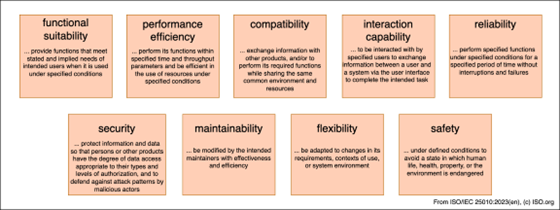
\includegraphics[width=0.85\textwidth]{iso25010.png}
  \caption{Overview on ISO 25010}
  \label{fig:iso25010}
\end{figure}

Hier ein Beispiel für eine Referenz, die dann auch automatisch aktualisiert:

In Figure~\ref{fig:iso25010}, we discuss \dots


\vspace{0.6cm}

\minititle{Motivation}
You should know the quality goals of your most important stakeholders, since they will influence fundamental architectural decisions. Make sure to be very concrete about these qualities, avoid buzzwords. If you as an architect do not know how the quality of your work will be judged\ldots

\minititle{Form}
A table with quality goals and concrete scenarios, ordered by priorities

\subsection{Stakeholders}

% Additional course comment:
% Add the stakeholder power matrix, and/or focus on change management if this is in the focus of your work.
% In any case, some description about the stakeholder universe should be added here.

\minititle{Contents}
Explicit overview of stakeholders of the system, i.e. all person, roles or organizations that
\begin{itemize}
  \item should know the architecture
  \item have to be convinced of the architecture
  \item have to work with the architecture or with code
  \item need the documentation of the architecture for their work
  \item have to come up with decisions about the system or its development
\end{itemize}

\minititle{Motivation}
You should know all parties involved in development of the system or affected by the system. Otherwise, you may get nasty surprises later in the development process. These stakeholders determine the extent and the level of detail of your work and its results.

\minititle{Form}
Table with role names, person names, and their expectations with respect to the architecture and its documentation.

\begin{longtable}{p{3cm} p{4cm} p{7cm}}
\toprule
Role/Name & Contact & Expectations \\
\midrule
\textless Role-1\textgreater & \textless Contact-1\textgreater & \textless Expectation-1\textgreater \\
\textless Role-2\textgreater & \textless Contact-2\textgreater & \textless Expectation-2\textgreater \\
\bottomrule
\end{longtable}

